\begin{titlepage}
\begin{center}

% Upper part of the page. The '~' is needed because only works if a paragraph has started.
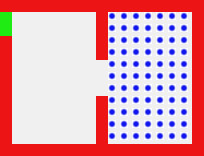
\includegraphics[width=.35\textwidth]{./titre/SimFoule0104}
%\caption{SiCF}
\label{fig:image1}
~\\[1cm]

\begin{figure}[htbp]
\begin{minipage}[c]{.45\linewidth}
\begin{center}
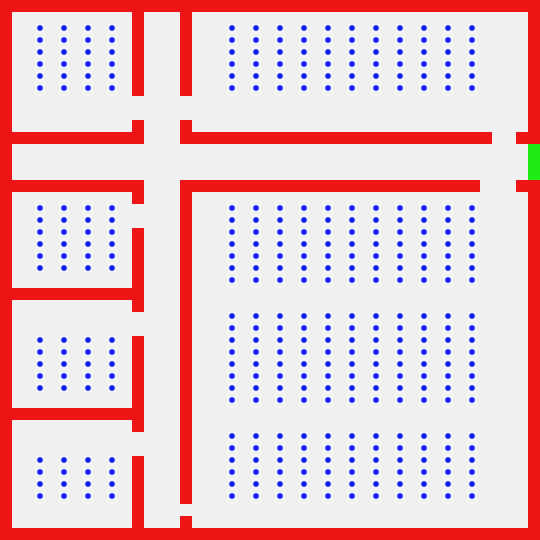
\includegraphics[scale=0.35]{./titre/SimFoule0103}
%\caption{SiCF}
%\label{fig:image1}
\end{center}
\end{minipage}
\hfill
\begin{minipage}[c]{.45\linewidth}
\begin{center}
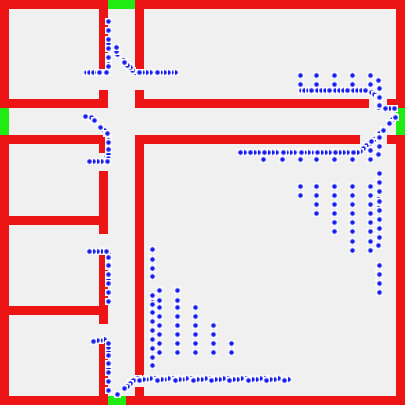
\includegraphics[scale=0.45]{./titre/SimFoule0105}
%\caption{diagramme des tâches.}
%\label{SiCP}
\end{center}
\end{minipage}
\end{figure}
%\textsc{\LARGE Complément nutritionnel}\\[1.5cm]
~\\[1cm]

\textsc{\Large }\\[0.5cm]

% Title
\HRule \\[0.4cm]

{\huge \bfseries  SimFoule 2.2\\[0.2cm] 
Documentation et théorie\\[0.4cm] }

\HRule \\[1.5cm]

% Author and supervisor
\begin{minipage}{0.4\textwidth}
\begin{flushleft} \large
%\emph{Auteur:}\\
%Stephan \textsc{Runigo}
\end{flushleft}
\end{minipage}
\begin{minipage}{0.4\textwidth}
\begin{flushright} \large
\emph{Auteur:}\\
Stephan \textsc{Runigo}
\end{flushright}
\end{minipage}

\vfill

% Bottom of the page
{\large \today}

\end{center}
\end{titlepage}
